\documentclass{article}

\usepackage[T2A]{fontenc}
\usepackage[utf8]{inputenc}
\usepackage[english, russian]{babel}

\usepackage{amssymb, amsmath, eucal, latexsym, amsthm}
\usepackage{epstopdf}
\usepackage{graphicx}
\usepackage{outlines}
\usepackage{mathrsfs}
\usepackage{xcolor}

\newtheorem*{theorem}{Теорема}
\newtheorem*{definition}{Определение}
\newtheorem{remark}{Замечание}

\newenvironment{psm}
	{\left( \begin{smallmatrix}}
	{\end{smallmatrix} \right) } 

\DeclareMathOperator*{\argmax}{arg\,max}

\begin{document}

\title{Теоремы о линейных операторах}

\maketitle

Рассматривается дифференциальное уравнение второго порядка с периодичной правой частью:
\begin{equation}
	u_{xx} = f(x, u), \quad f(x + L, u) = f(x, u).
\label{eq:initial}
\end{equation}
Функция $f(x, u)$ достаточно хорошая.
Периодичность правой части позволяется ввести отображение Пуанкаре $\mathcal{P}: \mathbb{R}^2 \to \mathbb{R}^2$ за период $L$, связанное с этим уравнением.
\begin{equation}
	\mathcal{P} \begin{pmatrix} u_0 \\ u_0' \end{pmatrix}
	= \begin{pmatrix} u_L \\ u_L' \end{pmatrix},
\end{equation}
где $u_L = u(L)$, $u_L' = u'(L)$, а $u(x)$ является решением уравнения \eqref{eq:initial} с начальными условиями $u(0) = u_0$, $u'(0) = u_0'$.
Отображение Пуанкаре $\mathcal{P}$, а также обратное к нему отображение $\mathcal{P}^{-1}$, могут быть определены не на всей фазовой плоскости $\mathbb{R}^2$, а лишь на некоторых её подмножествах.
Обозначим область определения отображения $\mathcal{P}$ за $\mathscr{U}_L^+$, а область определения отображения $\mathcal{P}$ за $\mathscr{U}_L^-$ соответственно.
Для дальнейшего изложения важно, чтобы совокупная область определения обоих отображений $\mathscr{U}_L = \mathscr{U}_L^+ \cap \mathscr{U}_L^-$ представляла из себя так называемое {\it островное множество}.

\begin{definition}
	Назовём {\bf островом} открытый криволинейный четырехугольник $D \subset \mathbb{R}^2$ на фазовой плоскости $(u, u')$, ограниченный двумя парами непересекающихся кривых $\alpha^{\pm}$, $\beta^{\pm}$, связанных с точками коллапса решений уравнения \eqref{eq:initial}, при этом:
	\begin{itemize}
		\item кривые $\alpha^{\pm}$ являются графиками монотонных $\gamma$-липшицевых функций $u' = h_{\pm}(u)$, а решение задачи \eqref{eq:initial} c начальными условиями $(u_0, u_0') \in \alpha^{\pm}$ коллапсирует в точке $x = -L$;
		\item кривые $\beta^{\pm}$ являются графиками монотонных $\gamma$-липшицевых функций $u = v_{\pm}(u')$, а решение задачи \eqref{eq:initial} c начальными условиями $(u_0, u_0') \in \beta^{\pm}$ коллапсирует в точке $x = +L$;
		\item если функции $h_{\pm}(u)$ являются возрастающими, тогда функции $v_{\pm}(u')$ -- убывающие, и наоборот, если функции $h_{\pm}(u)$ являются убывающими, тогда $v_{\pm}(u')$ -- возрастающие.
	\end{itemize}
\end{definition}

\begin{remark}
 	Решение задачи \eqref{eq:initial} с начальными условиями в точках пересечения кривых $\alpha^{\pm}$, $\beta^{\pm}$ коллапсирует как в точке $-L$, так и в точке $+L$.
\label{rem:alpha-beta-intersection}
\end{remark}

\begin{definition}
	Назовём множество $\mathcal{D} = \bigcup_{i \in S} D_i$, где $S$ конечное или счётное множество индексов, {\bf островным}, если оно представляет из себя конечное или счётное объединение взаимно непересекающихся островов, при этом выполняются следующие условия:
		\begin{itemize}
			\item[(а)] $\forall$ кривой $\Gamma \in D_i$, с конечными точками на границах острова $\beta_i^{\pm}$, пересечение $\mathcal{P} (\Gamma) \cap \beta_j^{\pm}$ непусто $\forall j$;
			\item[(б)] $\forall$ кривой $\Gamma \in D_i$, с конечными точками на границах острова $\alpha_i^{\pm}$, пересечение $\mathcal{P}^{-1} (\Gamma) \cap \alpha_j^{\pm}$ непусто $\forall j$.
		\end{itemize}
\end{definition}

\begin{figure}[h]
\centering
  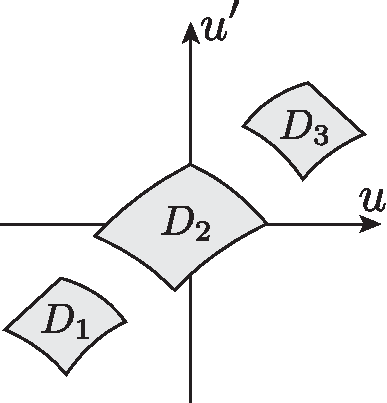
\includegraphics[scale = 0.8]{pic/set of islands}
  \caption{Пример островного множества $\mathcal{D}$ из 3-х островов.}
\label{fig:islands}
\end{figure}

На островном множестве $\mathcal{D}$ введем определения v,~h~-~кривых и v,~h~-~полос соответственно.

\begin{definition}
	Пусть $D \in \mathcal{D}$ -- остров, ограниченный кривыми $\alpha^{\pm}$, $\beta^{\pm}$.
	Рассмотрим кривую $\beta$, соединяющую противолежащие стороны $\alpha^{\pm}$ острова $D$.
	Назовём такую кривую {\bf v-кривой}, если она является графиком монотонной $\gamma$-липшицевой функции $u = v(u')$, при этом тип монотонности этой функции совпадает с типом монотонности функций $u = v_{\pm}(u')$ соответствующих границам $\beta^{\pm}$ острова $D$.
	Назовём {\bf v-полосой} открытое подмножество острова $D$, ограниченное двумя \emph{v}-кривыми.
\end{definition}

\begin{definition}
	Аналогично назовём кривую $\alpha$, соединяющую границы $\beta^{\pm}$, {\bf h-кривой}, если она является графиком монотонной $\gamma$-липшицевой функции $u' = h(u)$, при этом тип её монотонности совпадает с типом монотонности границ $\alpha^{\pm}$ острова $D$.
	Назовём {\bf h-полосой} открытое подмножество острова $D$, ограниченное двумя \emph{h}-кривыми.
\end{definition}

\begin{remark}
	Сам по себе остров является предельным случаем \emph{h} и \emph{v}-полосы одновременно.
\label{rem:island}
\end{remark}



\begin{figure}[h]
\centering
  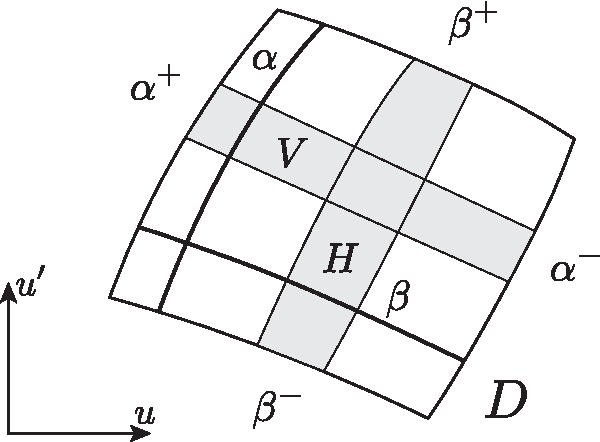
\includegraphics[scale = 0.8]{pic/curves and strips}
  \caption{Остров $D$ с границами $\alpha^+$, $\alpha^-$, $\beta^+$, $\beta^-$; h-кривая $\alpha$, v-кривая $\beta$, h-полоса $H$, v-полоса $V$.}
\label{fig:curves-and-strips}
\end{figure}

Введенные определения проиллюстрированы на рисунках \ref{fig:islands} и \ref{fig:curves-and-strips}.
Далее нам понадобится понятие ширины полос.
Ограничимся подробным изложением определений для h-полос.
Для v-полос все они записываются аналогичным образом.

Пусть h-полоса $H$ внутри острова $D$ ограничена кривыми $\alpha^+$, $\alpha^-$.
Рассмотрим графики этих кривых как функции от $u$; $\alpha^+$: $u' = h_+(u)$; $\alpha^-$: $u' = h_-(u)$.
Очевидно, что в силу геометрических особенностей острова, области определения функций $h_{\pm}(u)$ не совпадают, за исключением случая, когда границы острова $\beta^{\pm}$ являются вертикальными линиями.
Области определения функций $h_+$ и $h_-$ обозначим за $\Delta^+ = [u_0^+, u_1^+]$ и $\Delta^- = [u_0^-, u_0^+]$ соответственно.
Рассмотрим $\Delta = \Delta^+ \cup \Delta^-$ и доопределим функции $h_+$, $h_-$ на всём $\Delta$ следующим образом:
\begin{equation}
	\widetilde{h}_{\pm}(u) = \begin{cases}
		h_{\pm}(u_0^{\pm}) & u < u_0^{\pm}; \\
		h_{\pm}(u) & u \in \Delta^{\pm}; \\
		h_{\pm}(u_1^{\pm}) & u > u_1^{\pm}.
	\end{cases}
\end{equation}

В силу того, что функции $h_+$ и $h_-$ являются $\gamma$-липшицевыми на $\Delta^+$ и $\Delta^-$ соответственно, доопределённые функции $\widetilde{h}_+$ и $\widetilde{h}_-$ являются $\gamma$-липшицевыми на всём $\Delta$.
Полученные кривые обозначим за $\widetilde{\alpha}^+$ и $\widetilde{\alpha}^-$.

\begin{definition}
	Под {\bf шириной h-полосы}, ограниченной кривыми $\alpha^+$, $\alpha^-$, будем понимать расстояние между доопределёнными кривыми $\widetilde{\alpha}^+$, $\widetilde{\alpha}^-$ в смысле метрики пространства $\gamma$-липшицевых функций $C_{\gamma}(\Delta)$.
\end{definition}

\begin{remark}
 	Для двух h-полос $H_1$, $H_2$ верно $H_2 \subset H_1 \Rightarrow \Delta_2 \subseteq \Delta_1$.
\label{rem:h-strips}
\end{remark}

Для h-полосы $H$ с границами $\alpha^+$, $\alpha^-$ запишем выражение для её ширины:
\begin{equation}
	\rho(H) = \rho(\widetilde{\alpha}^+, \widetilde{\alpha}^-) = \max \limits_{u \in \Delta} |\widetilde{h}_+(u) - \widetilde{h}_-(u)|.
\label{eq:width-h-strip}
\end{equation}
Пусть максимум модуля разницы достигается в точке $u^*$, то есть
\begin{equation}
	u^* = \argmax \limits_{u \in \Delta} |\widetilde{h}_+(u) - \widetilde{h}_-(u)|.
\label{eq:argmax}
\end{equation}

\begin{definition}
	Будем говорить, что \emph{h}-полоса {\bf хорошо измерима}, если $u^* \in \Delta^+ \cap \Delta^-$.	
\end{definition}

\begin{remark}
	$\Delta^+ \cap \Delta^- \neq \varnothing \Rightarrow u^* \in \Delta^+ \cap \Delta^-$, то есть \emph{h}-полоса хорошо измерима, если области определения функций её границ имеют хотя бы одну общую точку. 
\end{remark}
\begin{proof}
	Данное утверждение непосредственно следует из монотонности границ h-полосы $\alpha^+$ и $\alpha^-$.
\end{proof}

\begin{remark}
	Любая \emph{h}-полоса, содержащаяся в хорошо измеримой \emph{h}-полосе, хорошо измерима.
\label{rem:well-h-strip}
\end{remark}

\begin{figure}[h]
\centering
  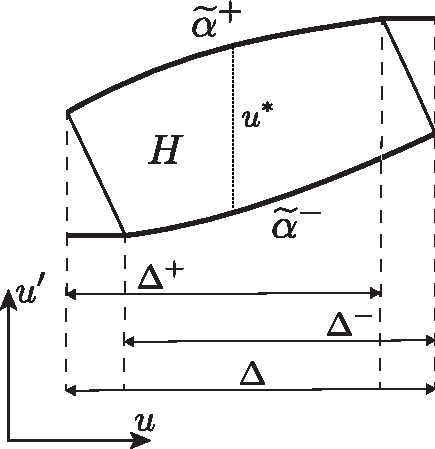
\includegraphics[scale = 0.8]{pic/width definition}
  \caption{Хорошо измеримая h-полоса $H$; доопределённые на весь интервал $\Delta$ границы $\widetilde{\alpha}^+$, $\widetilde{\alpha}^+$; точка $u^*$, в которой достигается максимум расстояния между границами, соответствует ширине полосы $H$.}
\label{fig:width-definition}
\end{figure}

Аналогичные определения вводят для v-полос подобным образом.
Введенное понятие ширины полос позволяет заменить лемму C.1 о пределе последовательности вложенных полос из оригинальной статьи \cite{ref:alfimov-avramenko-2013} полнотой пространства $\gamma$-липшицевых функций.
Понятие {\it хорошей} измеримости полос пригодится в доказательстве  нижеследующих теорем.
Оно означает, что ширину полосы можно измерить вдоль некоторой вертикальной (для h-полосы) или горизонтальной (для v-полосы) прямой, соединяющей точки с противоположных границ этой полосы.

Запишем линеаризацию отображения $\mathcal{P}$ в точке $p_0 = (u_0, u_0')$:
\begin{equation}
	\mathcal{P}(p) = \mathcal{P}_0 + D \mathcal{P}_0 (p - p_0) + o(||p - p_0||).
\label{eq:diff}
\end{equation}
Здесь $\mathcal{P}_0 = \mathcal{P}(p_0)$, а $J = D \mathcal{P}_0$ -- якобиан отображения $\mathcal{P}$ в точке $p_0$.
Линеаризация обратного отображения $\mathcal{P}^{-1}$ записывается аналогичным образом, при этом если $\mathcal{P}(p_0) = q_0$, тогда $(D \mathcal{P}_0)^{-1} = D \mathcal{P}_0^{-1}$, где $J^{-1} = D \mathcal{P}_0^{-1}$ -- якобиан обратного отображения $\mathcal{P}^{-1}$ в точке $q_0$.

Нижеследующая теорема устанавливает связь между свойствами матриц линейных операторов $D \mathcal{P}$, $D \mathcal{P}^{-1}$ и динамикой отображений $\mathcal{P}$, $\mathcal{P}^{-1}$ на фазовой плоскости.

\begin{theorem}[{\bf Об отображении h-полос}]

Пусть отображение Пуанкаре $\mathcal{P}$ и обратное к нему $\mathcal{P}^{-1}$ определены на островном множестве $\mathcal{D} = \bigcup_{i \in S} D_i$, где $S$ -- конечное или счетное множество индексов, при этом $\forall i, j \in S$ множество $V_{ji} = \mathcal{P}^{-1} D_j \cap D_i$ непусто, $\mathcal{P}$ определено на замыкании $\overline{V_{ji}}$, причём выполняется одно из двух условий:
\begin{enumerate}
	\item[(1)] границы $\alpha_i^{\pm}$ острова $D_i$ являются возрастающими кривыми, а знаки элементов матрицы линейного оператора $D \mathcal{P}_p = (a_{mn})$ имеют в каждой точке $p$ множества $\overline{V_{ji}}$ в точности одну из следующих конфигураций:
		\begin{center}
			(а) $\begin{psm} + & + \\ + & + \end{psm}$, \quad
			(б) $\begin{psm} - & - \\ - & - \end{psm}$, \quad
			(в) $\begin{psm} + & + \\ - & - \end{psm}$, \quad
			(г) $\begin{psm} - & - \\ + & + \end{psm}$;
		\end{center}
		при этом границы $\alpha_j^{\pm}$ острова $D_j$ являются возрастающими кривыми в случае (а), (б) и убывающими в случае (в), (г);
	\item[(2)] границы $\alpha_i^{\pm}$ острова $D_i$ являются убывающими кривыми, а знаки элементов матрицы линейного оператора $D \mathcal{P}_p = (a_{mn})$ имеют в каждой точке $p$ множества $\overline{V_{ji}}$ в точности одну из следующих конфигураций:
		\begin{center}
			(а) $\begin{psm} + & - \\ - & + \end{psm}$, \quad
			(б) $\begin{psm} - & + \\ + & - \end{psm}$,	\quad
			(в) $\begin{psm} + & - \\ + & - \end{psm}$, \quad
			(г) $\begin{psm} - & + \\ - & + \end{psm}$;		
		\end{center}
		при этом границы $\alpha_j^{\pm}$ острова $D_j$ являются убывающими кривыми в случае (а), (б) и возрастающими в случае (в), (г);
	\end{enumerate}
а также $\exists \mu > 1$ такое, что $\forall p \in \overline{V_{ji}}$, $|a_{11}| \ge \mu$, тогда $\forall$ h-полосы $H \in D_i$, $\forall j \in S$, $\mathcal{P} H \cap D_j = \widetilde{H}_j$ --- h-полоса, причем $\rho(\widetilde{H}_j) \le (1 / \mu) \rho(H)$.

\end{theorem}

\begin{proof}

Зафиксируем индексы $i, j$ и покажем, что утверждение теоремы выполняется для одной пары островов $D_i$, $D_j$.
По большей части проведём доказательство для случая (1.а).
Остальные случаи надлежит рассматривать полностью аналогичным образом.
Обозначим за $\mathbf{e}_1$, $\mathbf{e}_2$ базисные вектора
\begin{equation}
	\mathbf{e}_1 = \begin{pmatrix} 1 \\ 0 \end{pmatrix}; \quad \mathbf{e}_2 = \begin{pmatrix} 0 \\ 1 \end{pmatrix}.
\end{equation}
Определим следующий набор {\it конусов}:
\begin{align*}
	\mathbb{R}_{++}^2 = \{ \mathbf{v} \, | \, \mathbf{v} = x \mathbf{e}_1 + y \mathbf{e}_2, \; x > 0, y > 0 \}; \\
	\overline{\mathbb{R}}_{++}^2 = \{ \mathbf{v} \, | \, \mathbf{v} = x \mathbf{e}_1 + y \mathbf{e}_2, \; x \ge 0, y \ge 0 \}; \\
	\mathbb{R}_{+-}^2 = \{ \mathbf{v} \, | \, \mathbf{v} = x \mathbf{e}_1 + y \mathbf{e}_2, \; x > 0, y < 0 \}; \\
	\overline{\mathbb{R}}_{+-}^2 = \{ \mathbf{v} \, | \, \mathbf{v} = x \mathbf{e}_1 + y \mathbf{e}_2, \; x \ge 0, y \le 0 \}; \\
	\mathbb{R}_{-+}^2 = \{ \mathbf{v} \, | \, \mathbf{v} = x \mathbf{e}_1 + y \mathbf{e}_2, \; x < 0, y > 0 \}; \\
	\overline{\mathbb{R}}_{-+}^2 = \{ \mathbf{v} \, | \, \mathbf{v} = x \mathbf{e}_1 + y \mathbf{e}_2, \; x \le 0, y \ge 0 \}; \\
	\mathbb{R}_{--}^2 = \{ \mathbf{v} \, | \, \mathbf{v} = x \mathbf{e}_1 + y \mathbf{e}_2, \; x < 0, y < 0 \}; \\
	\overline{\mathbb{R}}_{--}^2 = \{ \mathbf{v} \, | \, \mathbf{v} = x \mathbf{e}_1 + y \mathbf{e}_2, \; x \le 0, y \le 0 \}. \\
\end{align*}
В качестве \underline{первого} шага доказательства заметим, что знаки матрицы линейного оператора $D \mathcal{P}_p = ( a_{mn} )$ однозначным образом определяют структуру отображения конусов в каждой точке $p$ множества $\overline{V_{ji}}$.
Для случая (а) имеем:
$$\forall \mathbf{v} = \begin{pmatrix} x \\ y \end{pmatrix} \in \overline{\mathbb{R}}_{++}^2, \ D \mathcal{P}_p(\mathbf{v}) = \begin{pmatrix} a_{11} & a_{12} \\ a_{21} & a_{22} \end{pmatrix} \begin{pmatrix} x \\ y \end{pmatrix} = \begin{pmatrix} \widetilde{x} > 0 \\ \widetilde{y} > 0\end{pmatrix} \in \mathbb{R}_{++}^2.$$
Несложно проверить, что полная схема отображения конусов для случая (1) теоремы выглядит следующим образом:
\begin{eqnarray*}
	(\textup{а}) & D \mathcal{P}_p (\overline{\mathbb{R}}_{++}^2) \in \mathbb{R}_{++}^2, \quad D \mathcal{P}_p (\overline{\mathbb{R}}_{--}^2) \in \mathbb{R}_{--}^2; \\
	(\textup{б}) & D \mathcal{P}_p (\overline{\mathbb{R}}_{++}^2) \in \mathbb{R}_{--}^2, \quad D \mathcal{P}_p (\overline{\mathbb{R}}_{--}^2) \in \mathbb{R}_{++}^2; \\
	(\textup{в}) & D \mathcal{P}_p (\overline{\mathbb{R}}_{++}^2) \in \mathbb{R}_{+-}^2, \quad D \mathcal{P}_p (\overline{\mathbb{R}}_{--}^2) \in \mathbb{R}_{-+}^2; \\
	(\textup{г}) & D \mathcal{P}_p (\overline{\mathbb{R}}_{++}^2) \in \mathbb{R}_{-+}^2, \quad D \mathcal{P}_p (\overline{\mathbb{R}}_{--}^2) \in \mathbb{R}_{+-}^2.
\end{eqnarray*}
Полная схема для случая (2) соответсвенно имеет следующий вид:
\begin{eqnarray*}
	(\textup{а}) & D \mathcal{P}_p (\overline{\mathbb{R}}_{-+}^2) \in \mathbb{R}_{-+}^2, \quad D \mathcal{P}_p (\overline{\mathbb{R}}_{+-}^2) \in \mathbb{R}_{+-}^2; \\
	(\textup{б}) & D \mathcal{P}_p (\overline{\mathbb{R}}_{-+}^2) \in \mathbb{R}_{+-}^2, \quad D \mathcal{P}_p (\overline{\mathbb{R}}_{+-}^2) \in \mathbb{R}_{-+}^2; \\
	(\textup{в}) & D \mathcal{P}_p (\overline{\mathbb{R}}_{-+}^2) \in \mathbb{R}_{--}^2, \quad D \mathcal{P}_p (\overline{\mathbb{R}}_{+-}^2) \in \mathbb{R}_{++}^2; \\
	(\textup{г}) & D \mathcal{P}_p (\overline{\mathbb{R}}_{-+}^2) \in \mathbb{R}_{++}^2, \quad D \mathcal{P}_p (\overline{\mathbb{R}}_{+-}^2) \in \mathbb{R}_{--}^2.
\end{eqnarray*}

\underline{Вторым} шагом покажем, что такое отображение конусов некоторым образом сохраняет свойства липшицевости и монотонности кривых из $\overline{V_{ji}}$ при отображении $\mathcal{P}$.
Продемонстрируем это на примере случая 1.(а).
Для начала заметим, что из компактности $\overline{V_{ji}}$ следует существование супремума
\begin{equation*}
	\widetilde{\gamma}_{ji} = \sup \dfrac{y}{x}, \ \begin{pmatrix} x \\ y \end{pmatrix} = D \mathcal{P}_p (\mathbf{v}), \ p \in \overline{V_{ji}}, \ \mathbf{v} \in \overline{\mathbb{R}}_{++}^2.
\end{equation*}
Далее пусть имеются две различные точки $p_1 \, p_2 \in \overline{V_{ji}}$, $p_1 = (\psi_1, \psi_1')$, $p_2 = (\psi_2, \psi_2')$, причём $\psi_2 \ge \psi_1$, $\psi_2' \ge \psi_2$.
Отображение $\mathcal{P}$ переводит точки $p_1$, $p_2$ в точки $q_1$, $q_2$ соответственно, $\mathcal{P}(p_1) = q_1 = (\phi_1, \phi_1')$, $\mathcal{P}(p_2) = q_2 = (\phi_2, \phi_2')$.
Пусть $D \mathcal{P}_1$ --- линеаризация отображения $\mathcal{P}$ в точке $p_1$.
Тогда справедливо следующее разложение:
\begin{equation}
	q_2 = \mathcal{P}(p_2) = q_1 + D \mathcal{P}_1 (p_2 - p_1) + r(||p_2 - p_1||),
\end{equation}
где $r(||p_2 - p_1||) / ||p_2 - p_1|| \to 0$ при $||p_2 - p_1|| \to 0.$
Вектор $\mathbf{p}_{\Delta} = p_2 - p_1 \in \overline{\mathbb{R}}_{++}^2$, а это означает, что его отображение оператором линеаризации $D \mathcal{P}_1 (\mathbf{p}_{\Delta}) = \mathbf{q}_{\Delta} \in \mathbb{R}_{++}^2$.
Таким образом
\begin{equation}
	q_2 - q_1 = \mathbf{q}_{\Delta} + r(||p_2 - p_1||),
\end{equation}
то есть для достаточно близких точек $p_1$, $p_2$ их образы $q_2 - q_1 \in \mathbb{R}_{++}^2$, то есть $\phi_2 > \phi_1$, $\phi_2' > \phi_1'$.
Более того можно выбрать $\gamma_{ji} > \widetilde{\gamma_{ji}}$ такое, что выполняется следующее неравенство:
\begin{equation}
	0 < \phi_2' - \phi_1' < \gamma_{ji} (\phi_2 - \phi_1).
\label{eq:ordering}
\end{equation}
Порядок, устанавливаемый соотношением \eqref{eq:ordering}, транзитивный, то есть из соотношения \eqref{eq:ordering} и второго аналогичного соотношения для достаточно близких точек $p_2$, $p_3$,
\begin{equation}
	0 < \phi_3' - \phi_2' < \gamma_{ji} (\phi_3 - \phi_2),
\end{equation}
следует аналогичное соотношение и для точке $p_1$, $p_3$.
Это позволяет распространить действие соотношения \eqref{eq:ordering} на любые точки $p_1, \, p_2 \in \overline{V_{ji}}$, для которых выполняется $\psi_2 \ge \psi_1$, $\psi_2' \ge \psi_1'$.
Остальные случаи рассматриваются аналогичным образом.

Таким образом в случае (1) теоремы для любых различных точек $p_1, \, p_2 \in \overline{V_{ji}}$, координаты которых связаны соотношением $\psi_2 \ge \psi_1$, $\psi_2' \ge \psi_1'$, для координат их образов $q_1 = (\phi_1, \phi_1'), \, q_2 = (\phi_2, \phi_2')$ в зависимости от знаков матрицы линеаризации $D \mathcal{P}_0$ выполняет одно из следующих неравенств ($\exists \gamma_{ji})$:
\begin{subequations}
\begin{eqnarray}
	(\textup{а}) & 0 < \phi_2' - \phi_1' < \gamma_{ji} (\phi_2 - \phi_1); \label{eq:ordering_1a} \\
	(\textup{б}) & 0 < \phi_1' - \phi_2' < \gamma_{ji} (\phi_1 - \phi_2); \label{eq:ordering_1b} \\
	(\textup{в}) & 0 < \phi_1' - \phi_2' < \gamma_{ji} (\phi_2 - \phi_1); \label{eq:ordering_1c} \\
	(\textup{г}) & 0 < \phi_2' - \phi_1' < \gamma_{ji} (\phi_1 - \phi_2). \label{eq:ordering_1d}
\end{eqnarray}
\end{subequations}
Для случая (2) теоремы в свою очередь имеем, что для любых различных точек $p_1, \, p_2 \in \overline{V_{ji}}$, координаты которых связаны соотношением $\psi_2 \le \psi_1$, $\psi_2' \ge \psi_1'$, выполняется одно из следующих неравенств:
\begin{subequations}
\begin{eqnarray}
	(\textup{а}) & 0 < \phi_2' - \phi_1' < \gamma_{ji} (\phi_1 - \phi_2); \label{eq:ordering_2a} \\
	(\textup{б}) & 0 < \phi_1' - \phi_2' < \gamma_{ji} (\phi_2 - \phi_1); \label{eq:ordering_2b} \\
	(\textup{в}) & 0 < \phi_1' - \phi_2' < \gamma_{ji} (\phi_1 - \phi_2); \label{eq:ordering_2c} \\
	(\textup{г}) & 0 < \phi_2' - \phi_1' < \gamma_{ji} (\phi_2 - \phi_1). \label{eq:ordering_2d}
\end{eqnarray}
\end{subequations}

\underline{Третьим} шагом продемонстрируем, как установленные выше неравенства позволяют заключить тот факт, что для любой h-полосы $H \in D_i$, её образ $\mathcal{P} H \cap D_j = \widetilde{H}_j$ также есть h-полоса.

Пусть полоса $H \in D_i$ расположена между двумя монотонными кривыми $\widetilde{\alpha}_i^{\pm}$, оконечные точки которых лежат на кривых $\beta_i^{\pm}$.
То есть $H$ есть криволинейных четырехугольник, ограниченный кривыми $\widetilde{\alpha}_i^{\pm}$ и сегментами кривых $\beta_i^{\pm}$.
Для случая (1.а) теоремы кривые $\widetilde{\alpha}_i^{\pm}$ являются возрастающими.
Рассмотрим образ кривой $\widetilde{\alpha}_i^+$.
Согласно определению островного множества $\mathcal{P} (\widetilde{\alpha}_i^+)$ пересекает каждую из границ $\beta_j^{\pm}$ острова $D_j$ хотя бы один раз.
При этом $\mathcal{P} (\widetilde{\alpha}_i^+)$ не может пересекать границы $\alpha_j^{\pm}$, поскольку они состоят из точек, образы которых уходят на бесконечность под действием $\mathcal{P}^{-1}$.

Пусть $\mathcal{P} (\widetilde{\alpha}_i^+)$ пересекает одну из границ $\beta_j^{\pm}$ острова $D_j$ дважды.
Обозначим эти точки пересечения за $q_1 = \mathcal{P}(p_1), \, q_2 = \mathcal{P}(p_2)$.
Для случая (1.а) границы $\alpha_j^{\pm}$ являются возрастающими кривыми, а $\beta_j^{\pm}$ --- убывающими, следовательно точки $q_1, \, q_2$ лежат не убывающей кривой.
Однако точки $p_1, \, p_2 \in \overline{V_{ji}}$ и лежат на возрастающей кривой $\widetilde{\alpha}_i^+$, следовательно для координат их образов $q_1 = (\phi_1, \phi_1'), \, q_2 = (\phi_2, \phi_2')$ должно выполнятся неравенство \eqref{eq:ordering_1a}.
А это означает, что точки $q_1, \, q_2$ лежать на убывающей кривой не могут.
Следовательно $\mathcal{P} (\widetilde{\alpha}_i^+)$ пересекает каждую границу $\beta_j^{\pm}$ лишь единожды.
Аналогичное утверждение верно и для $\mathcal{P} (\widetilde{\alpha}_i^-)$.

Таким образом $\mathcal{P} (\widetilde{\alpha}_i^{\pm}) \cap D_j$ есть монотонные кривые, тип монотонности которых совпадает с типом монотонности соответствующих границ острова $D_j$, причём эти кривые ограничивают множество $\mathcal{P} H \cap D_j$, следовательно $\mathcal{P} H \cap D_j = \widetilde{H}_j$ является h-полосой.
Остальные случаи теоремы рассматриваются полностью аналогичным образом, используя соотвествующие неравенства \eqref{eq:ordering_1a} -- \eqref{eq:ordering_1d}, \eqref{eq:ordering_2a} -- \eqref{eq:ordering_2d}.

Наконец \underline{четвертым} шагом доказательства покажем, что при введенном ограничении на значения $|a_{11}|$ оператора линеаризации $\forall H \in D_i$, $\rho (\widetilde{H}_j) \le \mu \rho(H)$, то есть ширина получаемой h-полосы внутри острова $D_j$ оказывается меньше ширины исходной полосы в острове $D_i$.

Для начала предположим, что h-полосы $H$ и $\widetilde{H}_j$ хорошо измеримы в смысле введенного выше определения.
Пусть полоса $\widetilde{H}_j$ измеряется вдоль вертикальной прямой, соединяющей точки $q_1 = (\phi_1, \phi_1'), \, q_2 = (\phi_2, \phi_2')$, $\phi_1' < \phi_2'$.
Рассмотрим параметризацию этой кривой $r(t) = (0, \phi'(t))$, где
\begin{equation}
	\phi'(t) = t \phi_2' + (1 - t) \phi_1', \quad 0 \le t \le 1.
\end{equation}
Поскольку полоса $\widetilde{H}_j$ хорошо измерима, $q(t) \in \widetilde{H}_j$.
Далее, $\widetilde{H}_j = \mathcal{P} H \cap D_j$, а значит существует прообраз кривой $p(t) = \mathcal{P}^{-1} (q(t)) = (\psi(t), \psi'(t))$, содержащийся внутри полосы $H$, то есть $q(t) = \mathcal{P} (p(t))$.
Для случая (1.а) нетрудно установить, что $p(t)$ является убывающей кривой, соединяющей точки с противолежащих границ $\widetilde{\alpha}_i^{\pm}$, ограничивающих полосу $H$ внутри острова $D_i$.
Действительно, поскольку кривая $q(t)$ содержится внутри некоего множества, которое в свою очередь является образом множества $\overline{V_{ji}}$, причем знаки в матрице линеаризации прямого отображения имеют вид $\begin{psm} + & + \\ + & + \end{psm}$, то знаки матрицы линеаризации обратного отображения $D \mathcal{P}^{-1}$ имеют вид $\begin{psm} + & - \\ - & + \end{psm}$ на кривой $q(t)$.
Это в свою очередь позволяет заключить соответствующее отображение конусов:
\begin{equation}
	D \mathcal{P}^{-1} \vert_{q(t)} (\overline{\mathbb{R}}_{-+}^2) \in \mathbb{R}_{-+}^2, \quad D \mathcal{P}^{-1} \vert_{q(t)} (\overline{\mathbb{R}}_{+-}^2) \in \mathbb{R}_{+-}^2.
\label{eq:cone-backward}
\end{equation}
Отображение конусов позволяет утверждать соответствующее свойство монотонности при отображении монотонных кривых аналогичное \eqref{eq:ordering_1a} -- \eqref{eq:ordering_1d}, из которого непосредственно следует, что вертикальная кривая $q(t)$ переходит в убывающую кривую $p(t)$.
Более того из неравенства $\phi_1' < \phi_2'$ при учете соответствующего отображения конусов в каждой точке следует, что $\psi'(t) > 0$.

\begin{figure}[h]
\centering
  \includegraphics[scale = 0.8]{pic/width of h-strip (a)}
  \caption{Иллюстрация к доказательству убывания ширины h-полос в случае, когда обе h-полосы $H$ и $\widetilde{H}_j$ хорошо измеримы. Ширина полосы $H$ измеряется вдоль пунктирной линии, ширина полосы $\widetilde{H}_j$ измеряется вдоль вертикальной прямой $q(t)$. Стрелочки указывают направление обхода кривых при изменении $t$ от $0$ до $1$.}
\label{fig:width-of-h-strip-a}
\end{figure}

Рассмотрим вектора, касательные к $p(t)$, $q(t)$:
\begin{eqnarray*}
	&& \dot{p}(t) = (\dot{\psi}(t), \dot{\psi}'(t)); \\
	&& \dot{q}(t) = (0, \dot{\phi}'(t)).
\end{eqnarray*}
В каждой точке $t$ эти вектора связаны между собой оператором линеаризации $D \mathcal{P} \vert_{p(t)}$
\begin{equation}
	\dot{q}(t) = D \mathcal{P} \vert_{p(t)} (\dot{p}(t)).
\end{equation}
Перепишем это соотношение в матричном виде:
\begin{equation}
	\begin{pmatrix}
		a_{11}(t) & a_{12}(t) \\ a_{21}(t) & a_{22}(t)
	\end{pmatrix}
	\begin{pmatrix}
		\dot{\psi}(t) \\
		\dot{\psi}'(t)
	\end{pmatrix} =
	\begin{pmatrix}
		0 \\ \dot{\phi}'(t)
	\end{pmatrix}.
\end{equation}
Принимая во внимание тот факт, что перед нами матрица линеаризации для отображения Пуанкаре, заключаем, что её определитель $a_{11}(t) a_{22}(t) - a_{12}(t) a_{21}(t) = 1$ в каждой точке $t$.
Из представленных выше соотношений и условия теоремы на значения $a_{11}(t)$ следует:
\begin{equation}
	\dot{\phi}'(t) = \dfrac{1}{a_{11}(t)} \dot{\psi}'(t) \le \dfrac{1}{\mu} \dot{\psi}'(t).
\end{equation}
Интегрируем полученное неравенство в пределах $0 \le t \le 1$, получаем:
\begin{equation}
	\rho(\widetilde{H}_j) = \phi_2' - \phi_1' = \int \limits_0^1 \dot{\phi}'(t) dt \le \dfrac{1}{\mu} \int \limits_0^1 \dot{\psi}'(t) dt = \dfrac{1}{\mu} (\psi_2' - \psi_1').
\end{equation}
Наконец, поскольку кривая $p(t)$ является убывающей, а границы полосы $H$ возрастающие кривые, из геометрических соображений следует тот факт, что $\psi_2' - \psi_1' \le \rho(H)$, то есть $\rho(\widetilde{H}_j) \le (1 / \mu) \rho(H)$.

Приведённое выше доказательство несложно обобщить на случаи, когда h-полосы $H$ и $\widetilde{H}_j$ не являются хорошо измеримыми.
Если полоса $H$ не является хорошо измеримой, неравенство $\psi_2' - \psi_1' \le \rho(H)$ все равно имеет место.
Это факт наглядно проиллюстрирован на Рис. \ref{fig:width-of-h-strip-b}.
Вертикальная разница между точками $p_1, \, p_2$ оказывает заведомо меньше ширины $H$ полосы.
\begin{figure}[h]
\centering
  \includegraphics[scale = 0.8]{pic/width of h-strip (b)}
  \caption{Иллюстрация к доказательству убывания ширины h-полос для случая, когда полоса $H$ не является хорошо измеримой. Её ширина измеряется вдоль пунктирной линии, одна из точек которой не принадлежит границе полосы $\alpha_i^+$.}
\label{fig:width-of-h-strip-b}
\end{figure}
В том случае, когда полоса $\widetilde{H}_j$ не является хорошо измеримой, следует соединить угловые точки $q_1, \, q_2$ монотонной убывающей кривой $q(t)$, как показано на Рис. \ref{fig:width-of-h-strip-c}, что всегда можно сделать согласно геометрическим свойствам h-полосы.
Опять же оказывается, что $\rho(\widetilde{H}_j) = \phi_2 - \phi_1$, а доказательство представленное выше также проходит, поскольку соответсвующее отображение конусов \eqref{eq:cone-backward} и следствия из него все также применимы для убывающий кривых $p(t)$, $q(t)$.
\begin{figure}[h]
\centering
  \includegraphics[scale = 0.8]{pic/width of h-strip (c)}
  \caption{Иллюстрация к доказательству убывания ширины h-полос для случая, когда полоса $\widetilde{H}_j$ не является хорошо измеримой.}
\label{fig:width-of-h-strip-с}
\end{figure}
Если обе h-полосы не являются хорошо измеримыми, тогда две описанные выше техники надлежит применить одновременно.

При рассмотрении остальных случаев теоремы изменяется лишь тип монотонности рассматриваемых объектов, а сама методика доказательства остается прежней и может быть применена аналогичным образом.
Теорема доказана.
\end{proof}

\pagebreak

\begin{theorem}[{\bf Об отображении v-полос}]
Пусть отображение Пуанкаре $\mathcal{P}$ и обратное к нему $\mathcal{P}^{-1}$ определены на островном множестве $\mathcal{D} = \bigcup_{i \in S} D_i$, где $S$ -- конечное или счётное множество индексов, при этом $\forall i, j \in S$ множество $H_{ij} = \mathcal{P} D_i \cap D_j$ непусто, $\mathcal{P}^{-1}$ определено на замыкании $\overline{H_{ij}}$, причём выполняется одно из двух условий:
\begin{enumerate}
	\item границы $\beta_i^{\pm}$ острова $D_i$ являются возрастающими кривыми, а знаки элементов матрицы линейного оператора $D \mathcal{P}_0^{-1} = (b_{mn})$ имеют в каждой точке $p$ множества $\overline{H_{ij}}$ в точности одну из следующих конфигураций:
		\begin{center}
			(а) $\begin{psm} + & + \\ + & + \end{psm}$, \quad
			(б) $\begin{psm} - & - \\ - & - \end{psm}$, \quad
			(в) $\begin{psm} + & + \\ - & - \end{psm}$, \quad
			(г) $\begin{psm} - & - \\ + & + \end{psm}$;
		\end{center}
		при этом границы $\beta_j^{\pm}$ острова $D_j$ являются возрастающими кривыми в случае (а), (б) и убывающими в случае (в), (г);
	\item границы $\beta_i^{\pm}$ острова $D_i$ являются убывающими кривыми, а знаки элементов матрицы линейного оператора $D \mathcal{P}_0^{-1} = (b_{mn})$ имеют в каждой точке $p$ множества $\overline{H_{ij}}$ в точности одну из следующих конфигураций:
		\begin{center}
			 (а) $\begin{psm} + & - \\ - & + \end{psm}$, \quad
			 (б) $\begin{psm} - & + \\ + & - \end{psm}$, \quad
			 (в) $\begin{psm} + & - \\ + & - \end{psm}$, \quad
			 (г) $\begin{psm} - & + \\ - & + \end{psm}$;
		\end{center}
		при этом границы $\beta_j^{\pm}$ острова $D_j$ являются убывающими кривыми в случае (а), (б) и возрастающими в случае (в), (г);
\end{enumerate}
а также $\exists \nu > 1$ такое, что $\forall p \in \overline{H_{ij}}$, $|b_{22}| \ge \nu$, тогда $\forall$ v-полосы $V \in \mathcal{D}$, $\forall i \in S$, $\mathcal{P}^{-1} V \cap D_i = \widetilde{V}_i$ -- v-полоса, причем $\rho(\widetilde{V}_i) \le (1 / \nu) \rho(V)$.

\end{theorem}

\begin{proof}
	Полностью аналогично доказательству теоремы об отображении h-полос.
\end{proof}

\section*{Приложения}

\paragraph{Случай общего положения.} 

Можно просканировать фазовую плоскость с некоторым шагом и просчитать матрицы линейного оператора на множествах $\mathcal{P} D_i \cap D_j$ и $\mathcal{P}^{-1} D_i \cap D_j$, $\forall i, j$.

\paragraph{Асимптотический предел.}

Области определения внутри островов оказываются вмонтированы в асимптотические разложения.
Можно исследовать матрицы линейного оператора в асимптотическом пределе для каждой пары островов $D_i$, $D_j$.

\begin{thebibliography}{99}
\bibitem{ref:alfimov-avramenko-2013} G.~L.~Alfimov, A.~I.~Avramenko, Coding of nonlinear states for the Gross-Pitaevskii equation with periodic potential, Physica D 254 (2013) 29-45.
\end{thebibliography}

\end{document}
